
%(BEGIN_QUESTION)
% Copyright 2012, Tony R. Kuphaldt, released under the Creative Commons Attribution License (v 1.0)
% This means you may do almost anything with this work of mine, so long as you give me proper credit

Calculate the buoyant force exerted on this level instrument's displacer at the following percentages of span.  Assume a cylindrical displacer with a diameter of 2 inches:

$$\includegraphics[width=15.5cm]{i02795x01.eps}$$

% No blank lines allowed between lines of an \halign structure!
% I use comments (%) instead, so that TeX doesn't choke.

$$\vbox{\offinterlineskip
\halign{\strut
\vrule \quad\hfil # \ \hfil & 
\vrule \quad\hfil # \ \hfil \vrule \cr
\noalign{\hrule}
%
% First row
Percent of & Buoyant  \cr
%
% Another row
span (\%) & force (lb) \cr
%
\noalign{\hrule}
%
% Another row
0 &  \cr
%
\noalign{\hrule}
%
% Another row
35 &  \cr
%
\noalign{\hrule}
%
% Another row
100 &  \cr
%
\noalign{\hrule}
} % End of \halign 
}$$ % End of \vbox

\underbar{file i02795}
%(END_QUESTION)





%(BEGIN_ANSWER)

% No blank lines allowed between lines of an \halign structure!
% I use comments (%) instead, so that TeX doesn't choke.

$$\vbox{\offinterlineskip
\halign{\strut
\vrule \quad\hfil # \ \hfil & 
\vrule \quad\hfil # \ \hfil \vrule \cr
\noalign{\hrule}
%
% First row
Percent of & Buoyant  \cr
%
% Another row
span (\%) & force (lb) \cr
%
\noalign{\hrule}
%
% Another row
0 & 0 \cr
%
\noalign{\hrule}
%
% Another row
35 & 0.4550 \cr
%
\noalign{\hrule}
%
% Another row
100 & 1.300 \cr
%
\noalign{\hrule}
} % End of \halign 
}$$ % End of \vbox


%(END_ANSWER)





%(BEGIN_NOTES)

{\bf This question is intended for exams only and not worksheets!}.

%(END_NOTES)


